\section{评测}
为全面评估 Baichuan-M3 的临床效用与安全性，我们在两个互补维度上进行严格实验：动态临床流程模拟（\textbf{ScanBench}）与广谱医学推理（\textbf{HealthBench}~\cite{healthbench}）。我们将 Baichuan-M3 与多种有竞争力的基线进行对比，以确保评估的稳健性。这些基线包括推理能力突出的通用大模型（如 \textbf{GPT-5.2-High}\cite{openai2025gpt52}、\textbf{Deepseek-V3.2-Thinking}\cite{deepseek2025v32thinking}、\textbf{Qwen3-235B-thinking-2507}\cite{qwen3-235b-thinking-2507}）、代表性的医疗专用模型（如 \textbf{AntAngelMed}\cite{antangelmed2026}）以及上一代模型（\textbf{Baichuan-M2}~\cite{baichuan-m2}）。关键的是，为与真实专业标准对齐，我们引入由三甲医院主治医师组成的人类基线，每位医生至少具有 5 年临床经验。该对比分析旨在验证模型在复杂决策、专业知识应用与幻觉抑制方面相较通用大模型、领域模型与人类专家的进步。

\subsection{ScanBench}
不同于传统静态问答基准，ScanBench 模拟真实临床流程“问诊 $\rightarrow$ 检验检查 $\rightarrow$ 诊断”。该数据集计划开源，将多样临床病例转化为可观测、可量化的决策路径，并划分为三个渐进阶段。

\subsubsection{数据集构成与统计}
ScanBench 从病例多样性、问诊粒度与检查复杂度三个维度高保真地模拟真实临床环境。

\paragraph{临床病例多样性}
如表~\ref{tab:scanbench_distribution} 所示，ScanBench 包含来自 12 个科室的 303 个病例，覆盖常见疾病（如全科）与长尾专科（如风湿科、血液科）。

\begin{table}[H]
\centering
\caption{按科室划分的临床样本分布。}
\label{tab:scanbench_distribution}
\begin{tabular}{lclc} % Compacted the table slightly
\toprule
\textbf{Department} & \textbf{Count} & \textbf{Department} & \textbf{Count} \\ \midrule
General Practice    & 111 & Nephrology           & 15 \\
Surgery             & 50  & Cardiology           & 14 \\
Gynecology          & 26  & Respiratory Medicine & 14 \\
Neurology           & 25  & Endocrinology        & 7  \\
Gastroenterology    & 18  & Rheumatology         & 6  \\
Hematology          & 15  & Geriatrics           & 2  \\ \bottomrule
\end{tabular}
\end{table}

\paragraph{问诊粒度与严谨性}
为量化问诊过程，我们标注了 8,857 条清单项作为真值。
\begin{itemize}
    \item \textbf{信息密度：} 每个病例平均包含 29.23 项（范围：20--35），需要持续的多轮上下文跟踪。
    \item \textbf{逻辑分布：} 清单反映临床诊断逻辑：现病史占比最高（55.8\%），其次为既往史（19.6\%）与个人/社会史（14.6\%），并在相关时包含产科/妇科史（5.4\%）与家族史（4.7\%）。
    \item \textbf{关键性权重：} 我们区分关键安全要点与一般信息：51.3\% 标注为 Level 2（关键），用于诊断与风险排除，其余 48.7\% 为 Level 1（补充）。
\end{itemize}

\paragraph{综合检查动作空间}
在辅助检查阶段，模型在 38 个类别的统一动作空间内进行选择，模拟真实医院的资源管理复杂度，包括：
\begin{itemize}
    \item \textbf{常规与生化：} 血/尿/便常规、肝肾功能、电解质、CRP、糖代谢（含 OGTT/HbA1c）等。
    \item \textbf{影像与功能：} CT、MRI、超声、X 光、心电图、脑电图、肺功能等。
    \item \textbf{病理与专科：} 肿瘤标志物、病毒标志物、自身抗体、激素、骨髓活检、内镜等。
\end{itemize}
这一丰富的候选集要求模型在避免资源浪费的同时精准选择必要检查。

\subsubsection{流程与评估方法}
评估流程始于站点 1：问诊，模型与标准化病人进行多轮互动。为评估过程质量，我们引入 SCAN 框架，将问诊表现分解为四个维度：风险分层（Safety Stratification）、信息澄清（Information Clarification）、关联性提问（Associative Questioning）与规范化输出（Normative Output）。我们使用 GPT-4.1~\cite{gpt4} 验证 OSCE 关键临床要点的覆盖度，同时剔除每次问诊中反复出现且非诊断性的内容（如反复陈述年龄/性别或模板化自我介绍）。

% Given the elicited evidence, Station 2: Lab Testing evaluates both resource efficiency and interpretative accuracy. The model proposes a differential diagnosis and selects laboratory or imaging tests from a unified candidate pool. Performance is measured by F1 against a physician-curated ground-truth set, reflecting the trade-off between ordering precision and recall.

在已获得证据的基础上，站点 2：检验检查评估资源效率与解读准确性。模型提出鉴别诊断并从统一候选池中选择检验或影像检查，候选检查根据对诊断与决策的贡献被划分为“必需”与“可选”。性能采用加权 F1 评估，其中对必需检查的召回赋予更高权重，以体现其在诊断流程中的重要性，同时保持整体精确率与覆盖率的平衡评价。

流程在站点 3：诊断结束，模型整合所有先验信息做出最终诊断。我们采用基于 ICD-10 分类的层级匹配标准：正确命中叶子节点得到奖励，分支偏离则受到惩罚。


\subsubsection{性能分析}

如图~\ref{fig:scan_bench_main} 所示，Baichuan-M3 在三大站点均排名第一，展现出全面优势。尤其在最具挑战的临床问诊阶段，得分 74.9，较第二名 GPT-5.2-High 高出 12.4 分，并超过人类基线 20 分以上。这一优势同样体现在检验检查（72.1）与最终诊断（74.4）上，表明 Baichuan-M3 具备稳健的端到端医学推理能力，而非仅在孤立任务上表现突出。

\begin{figure}[H]
    \centering
    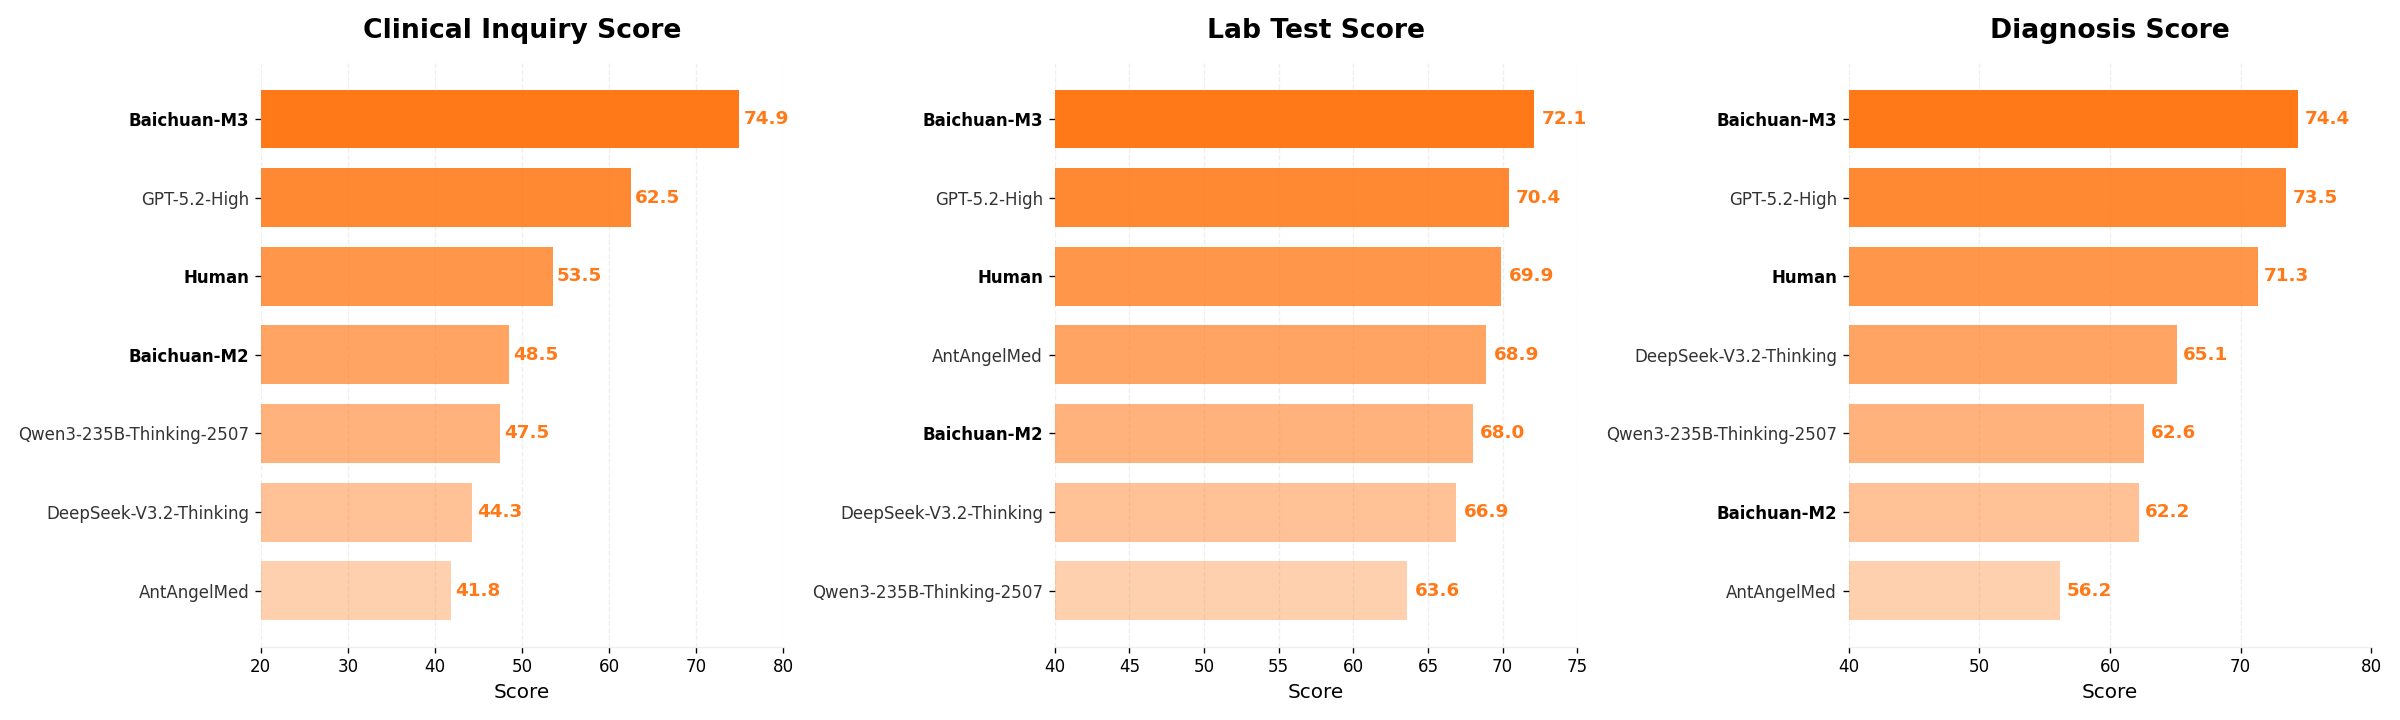
\includegraphics[width=1.0\linewidth]{image/scan_1x3.png}
    \caption{ScanBench 总体性能对比。}
    \label{fig:scan_bench_main}
\end{figure}


使用 SCAN 框架对问诊能力进行进一步拆解（图~\ref{fig:scan_bench_dims}），Baichuan-M3 是唯一在四个维度上均展现显著领先的模型，持续超越 SOTA 大模型与人类专家。

具体而言，在风险分层方面，Baichuan-M3 取得 75.8 的高分，显著领先第二名 Qwen3-235B（48.3），几乎是人类基线（40.1）的两倍。这表明其对“红旗”症状与关键风险具有更高敏感性。在关联性提问方面，得分 72.6，显著超过 GPT-5.2-High（54.5），体现其对鉴别诊断的精细把握，能够主动挖掘超越用户初始描述的潜在线索。此外，Baichuan-M3 在清晰度（84.5）与规范化流程（59.9）上表现突出，保证收集信息既细致又结构化标准化。综合这些优势，Baichuan-M3 构建了精确问诊与安全决策的闭环，标准化水平超过人类基线。

\begin{figure}[H]
    \centering
    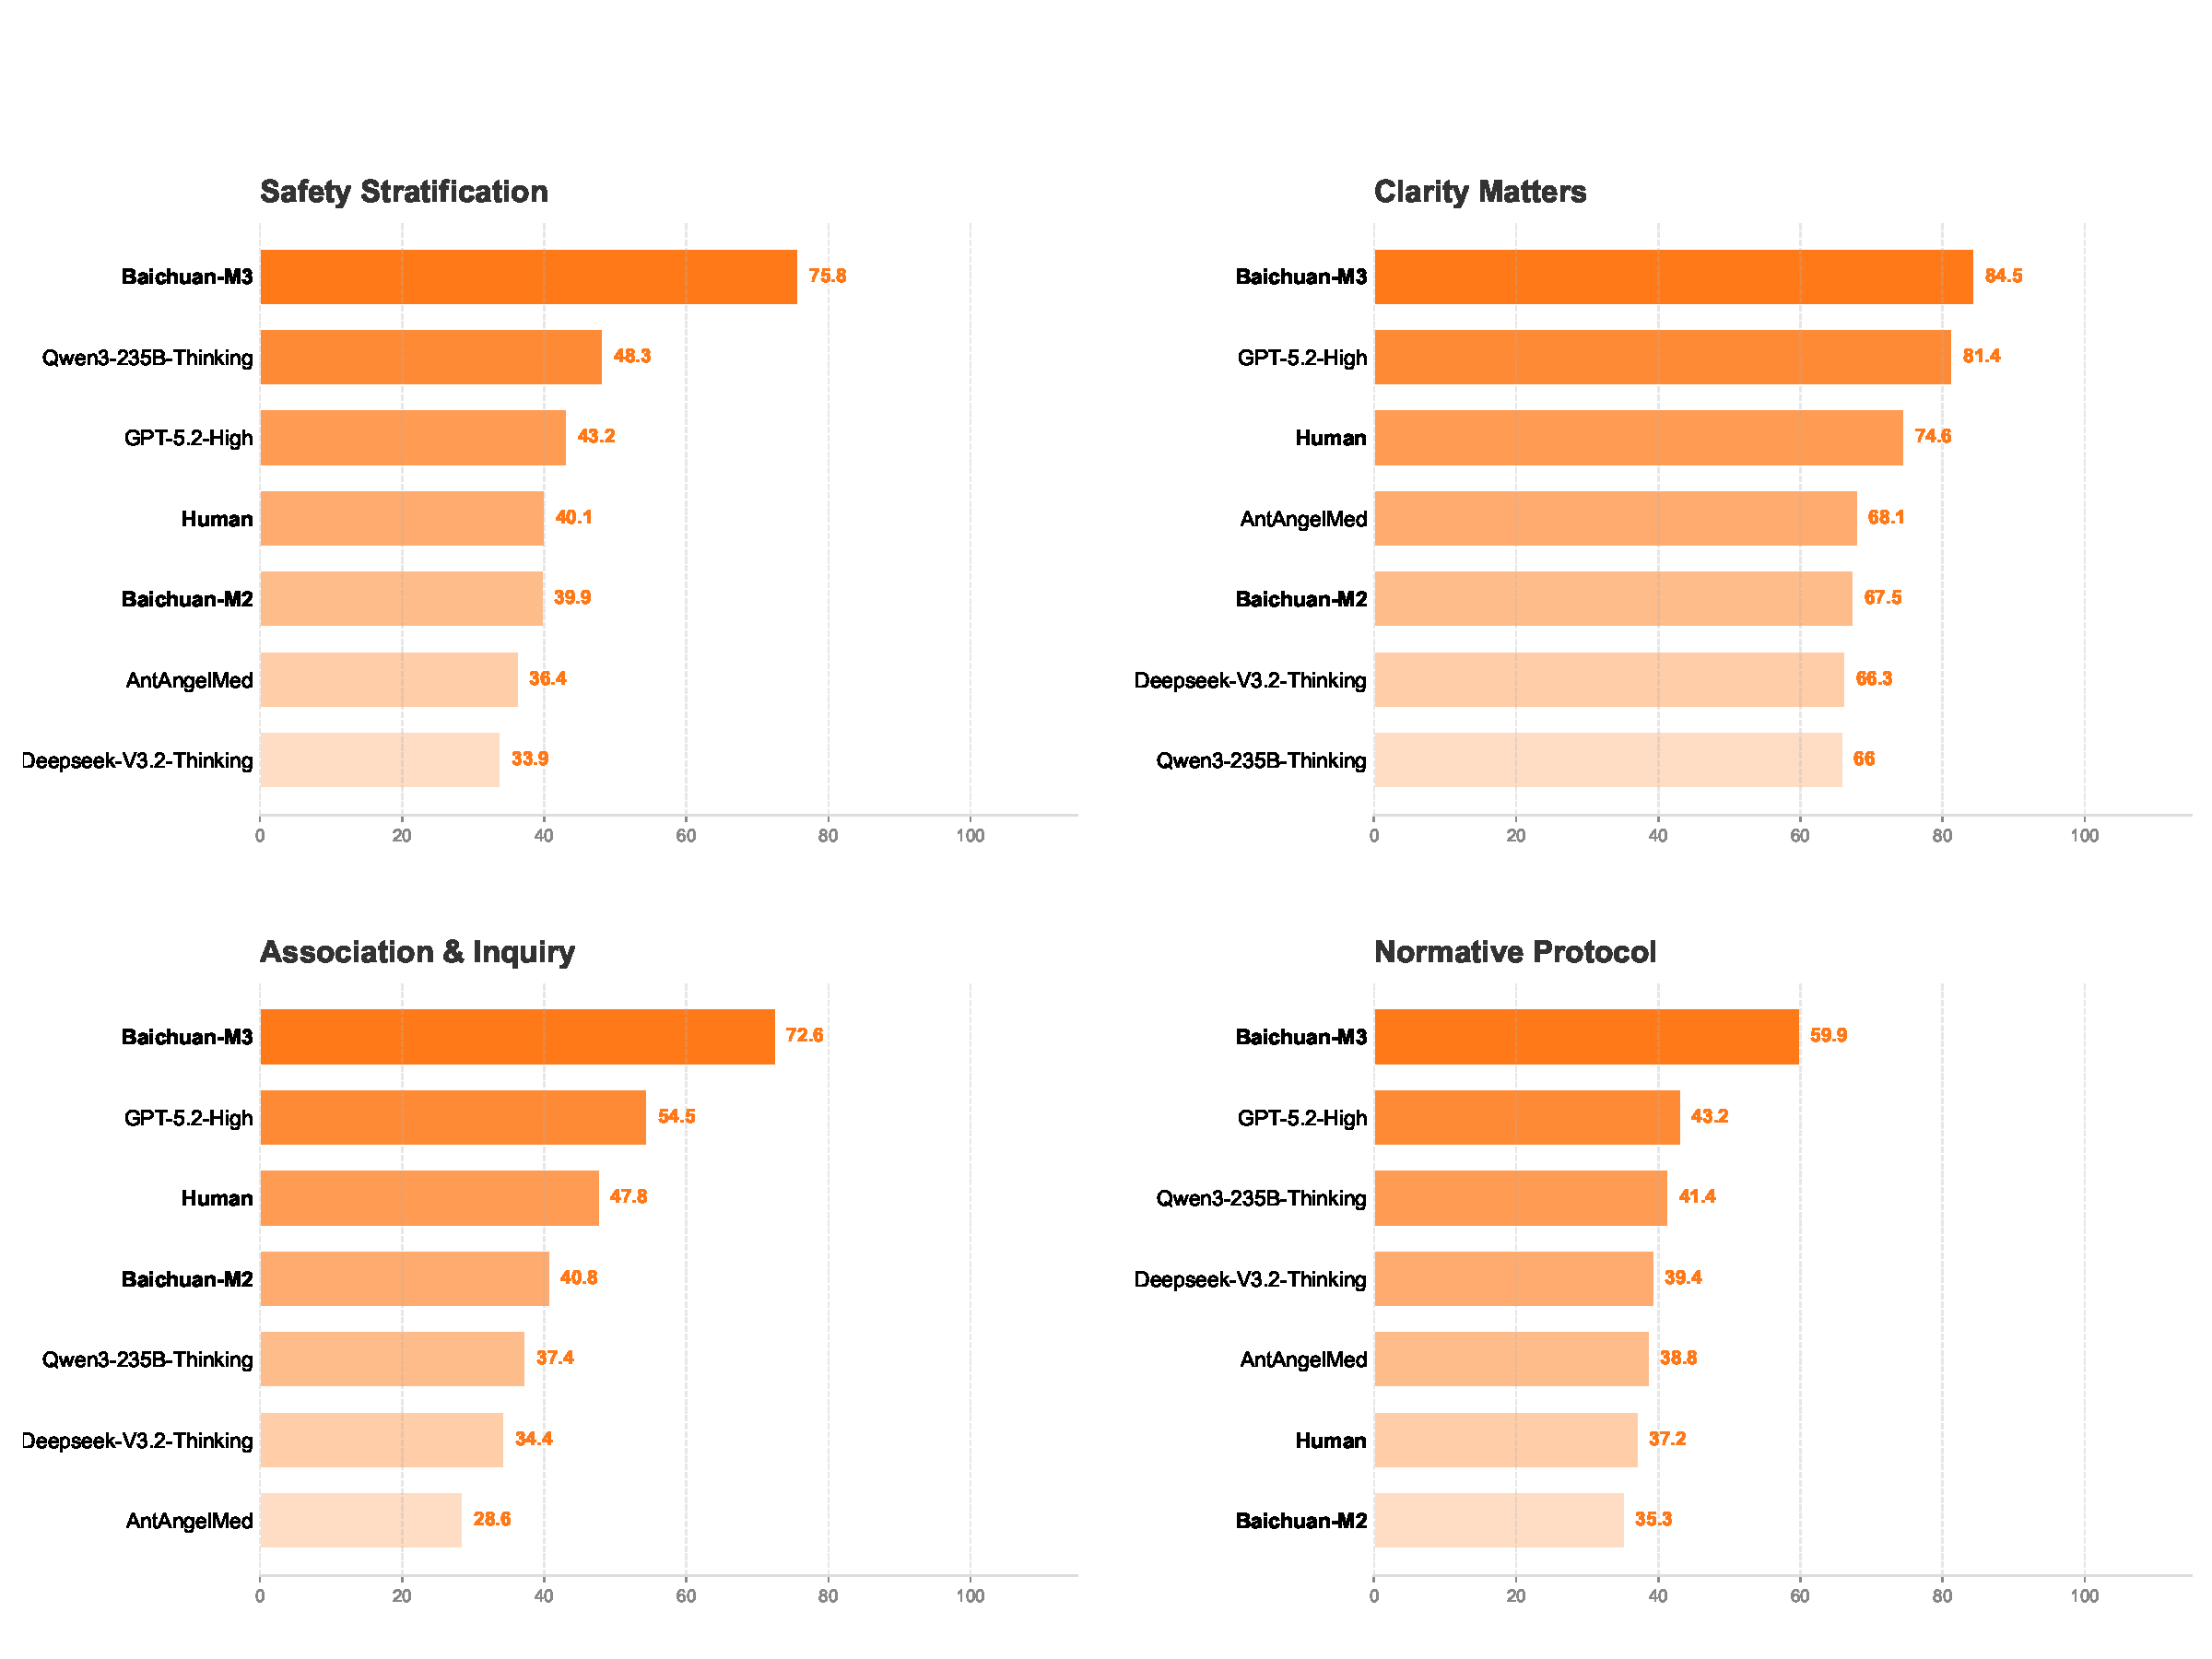
\includegraphics[width=1.0\linewidth]{image/scan_2x2.pdf}
    \caption{问诊能力的细粒度拆解。}
    \label{fig:scan_bench_dims}
\end{figure}


\subsubsection{动态问诊效率}
图~\ref{fig:scan_turn_evlo} 展示了模型分数随对话轮次变化的趋势。为减少极少数超长对话带来的噪声，我们剔除样本占比低于 10\% 的轮次区间，使趋势更易解读。


\paragraph{基础收敛，推理分化}
图~\ref{fig:scan_turn_evlo}b 显示，大多数模型在症状澄清上很快达到相近水平（约 0.7--0.8）。差距在关联性提问上逐渐显现（图~\ref{fig:scan_turn_evlo}c）：Baichuan-M3 随对话推进持续提升，而通用模型（如 Deepseek 与 Qwen）逐渐落后——在长时程场景形成近乎两倍的优势。

\paragraph{风险敏感性与上下文遵循}
在风险分层方面（图~\ref{fig:scan_turn_evlo}a），Baichuan-M3 对风险信号更敏感，随证据累积得分上升至约 0.7。相比之下，GPT-5.2-High 即使在较长对话中也徘徊在 0.5 左右，显示急性风险识别能力较弱。在规范化流程方面（图~\ref{fig:scan_turn_evlo}d），模型表现随轮次提升而提高，表明保持上下文有助于遵循结构化临床流程。

\begin{figure}[H]
    \centering
    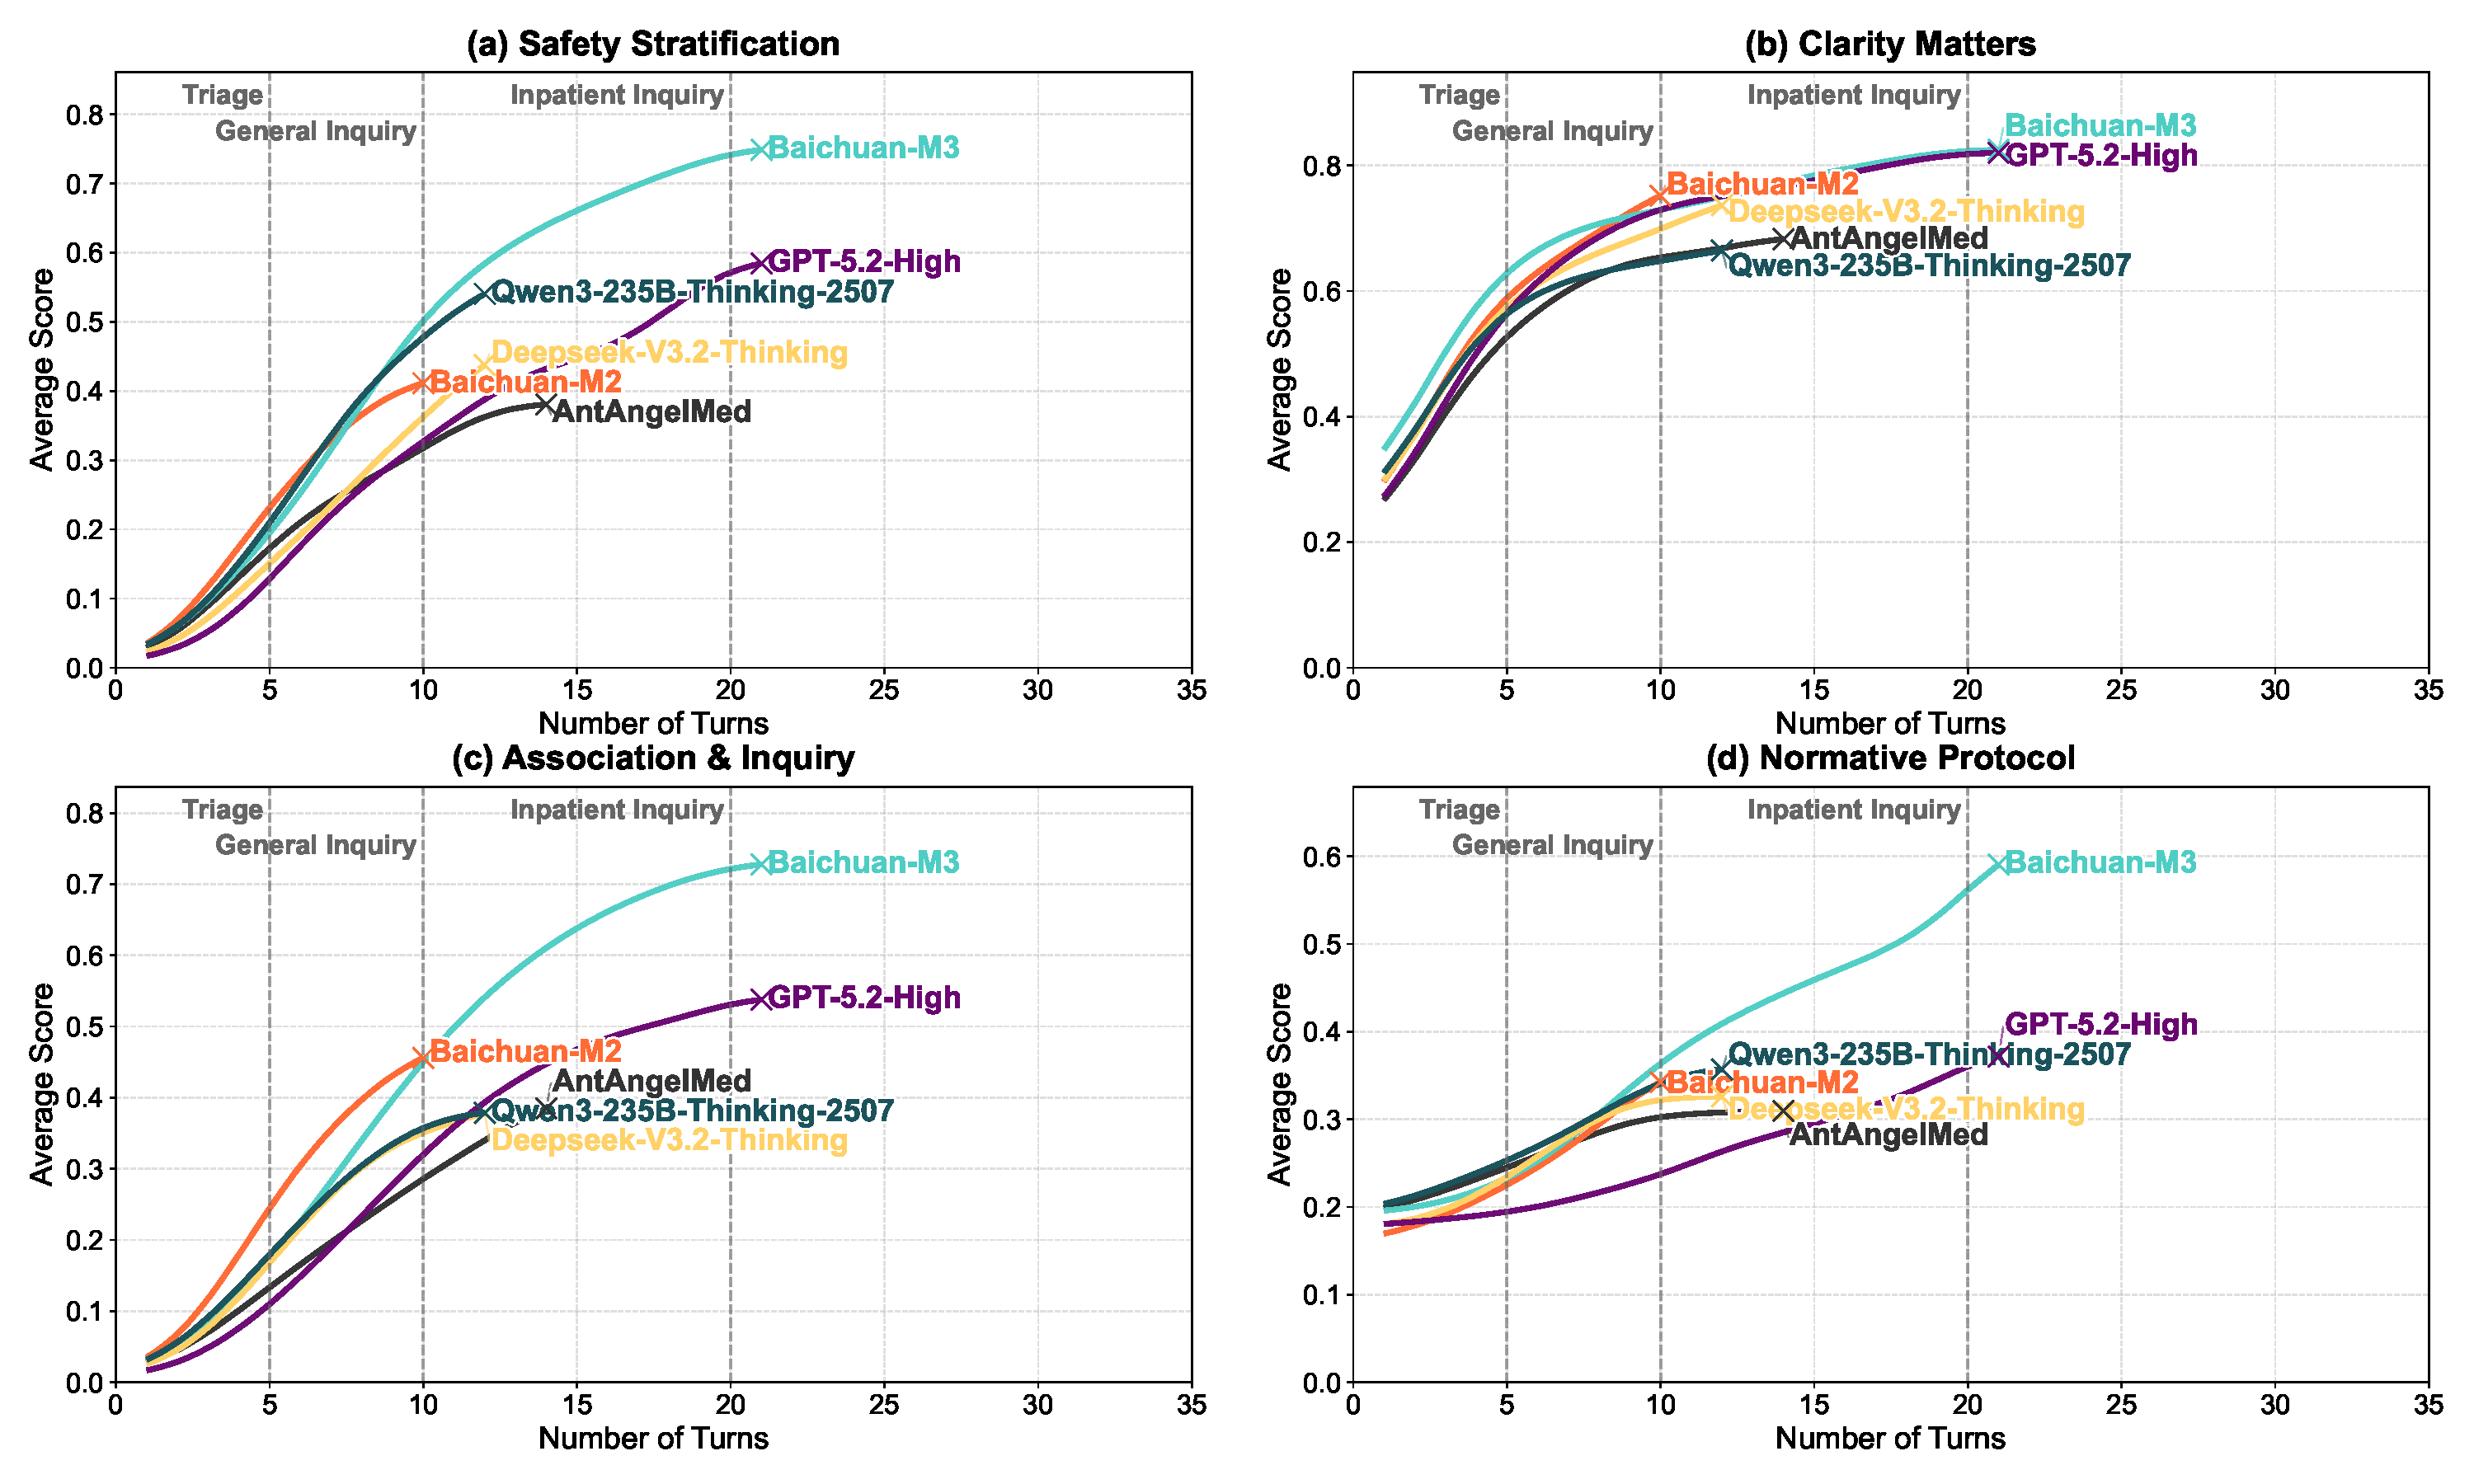
\includegraphics[width=0.95\linewidth]{image/merged_metrics_SCAN.pdf}
    \caption{模型性能随对话轮次的演化。}
    \label{fig:scan_turn_evlo}
\end{figure}


总之，通用 LLM 可满足基础信息采集，但临床场景所需的复杂推理与安全保障仍离不开专门训练。


\subsection{HealthBench}
% 1. 引言部分：只介绍 Bench 本身
HealthBench 是评估 LLM 临床推理能力与安全边界的严格基准。通过在不同难度与维度上评估性能，它提供了模型在真实医疗场景中效用的全面视角。

\subsubsection{HealthBench-Main}
% 2. 第一段：Overall Performance (SOTA 对比)
如图~\ref{fig:exp_hb} 所示，\textbf{Baichuan-M3} 在所有关键指标上建立了新的 SOTA 标准。在综合 \textit{HealthBench Total} 上，Baichuan-M3 得分 \textbf{65.1}，明显超过亚军 GPT-5.2-High（63.3）。在高难度 \textit{HealthBench Hard} 子集上，Baichuan-M3 进一步扩大领先优势，得分 \textbf{44.4}，显著超过 GPT-5.2-High（42.0）与 AntAngelMed（39.6）。此外，Baichuan-M3 以 \textbf{3.5\%} 的最低\textit{幻觉率}展现出卓越可靠性，表明其在深度临床推理与事实准确性之间取得了更稳健的平衡。

\begin{figure}[H]
    \centering
    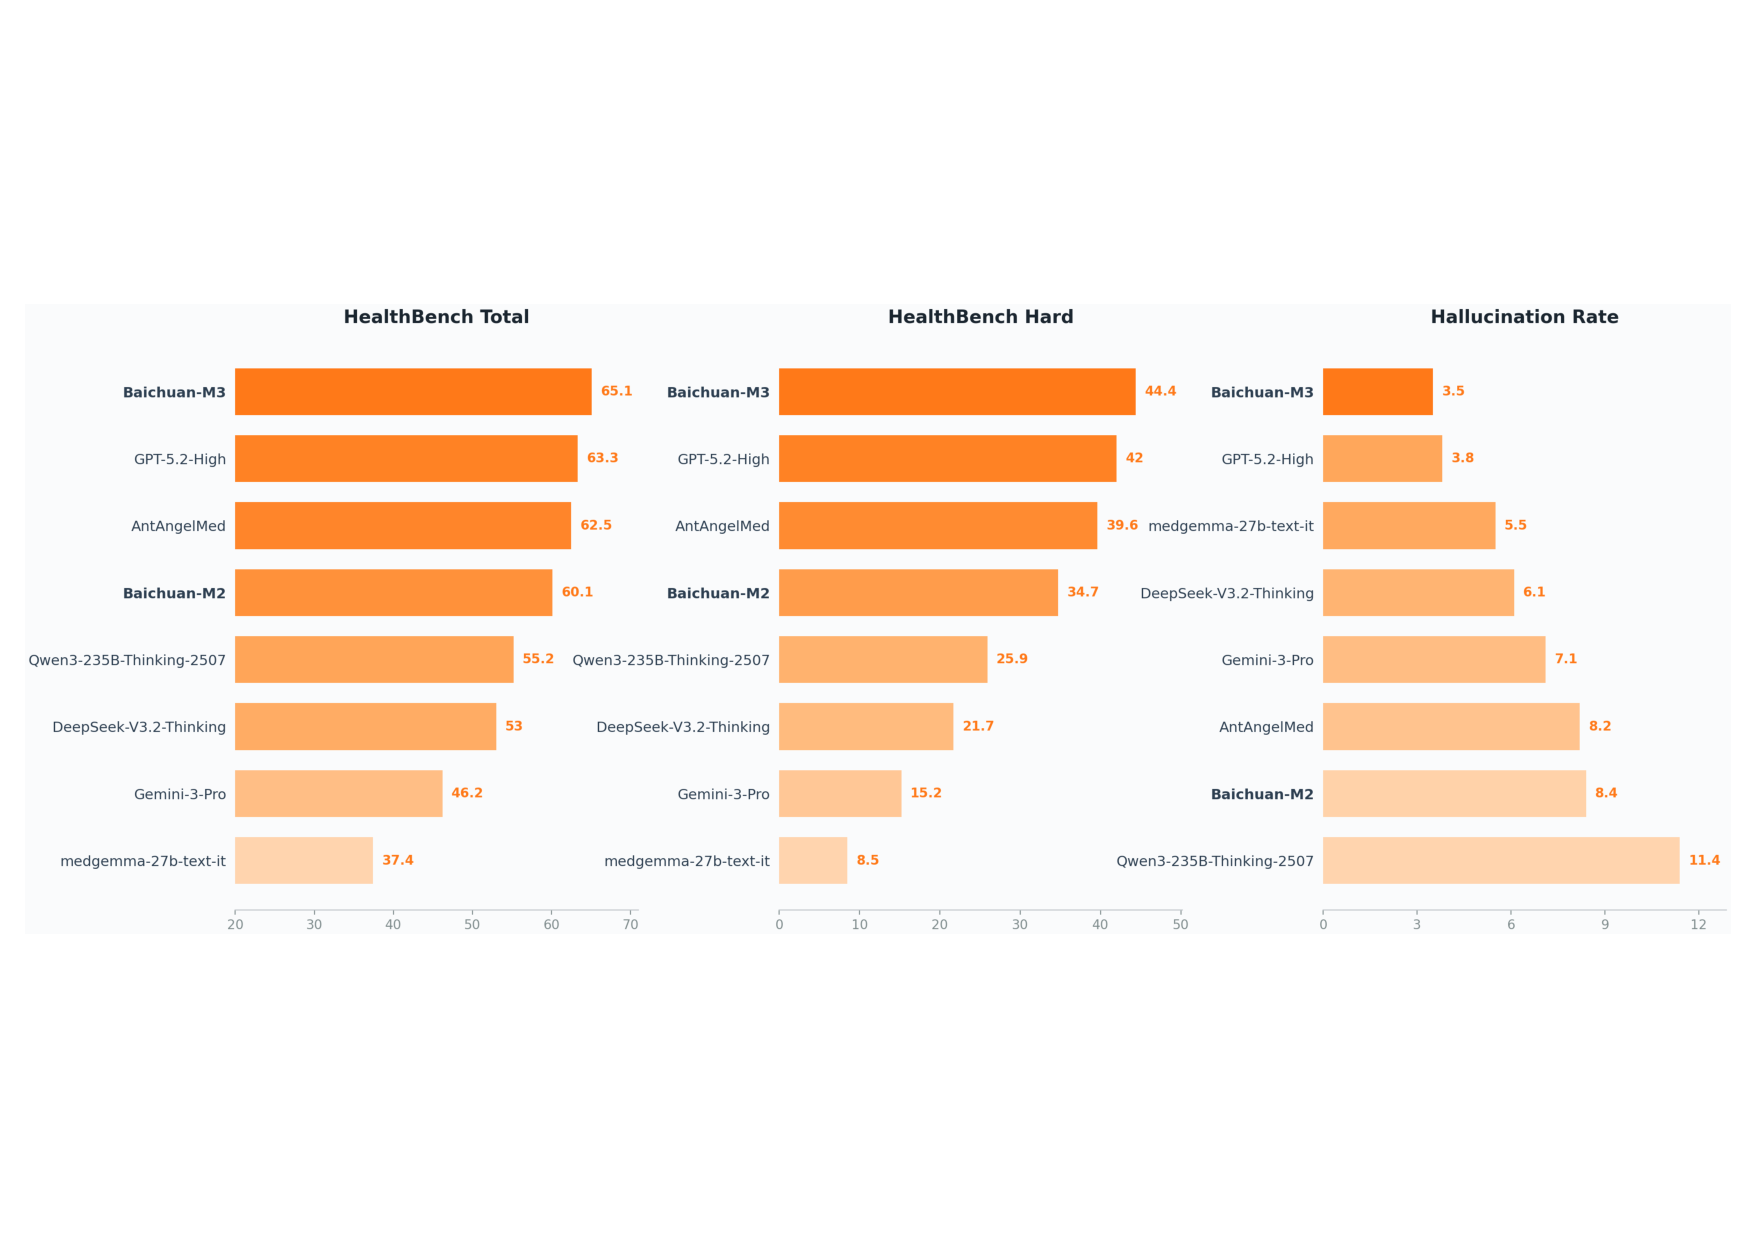
\includegraphics[width=0.98\linewidth]{image/healthbench.pdf}
    \caption{HealthBench 总体性能对比。}
    \label{fig:exp_hb}
\end{figure}

% 3. 第二段：Fine-grained Analysis (M2 vs M3 对比)
与 M2 相比，M3 在大多数评估维度上均有广泛提升，从而形成更稳健、均衡的医疗服务能力画像（见图~\ref{fig:hb_m2_m3}）。提升尤以“上下文寻求”与“上下文感知”为显著。我们将这些增益归因于深度临床问诊训练的迁移：M3 更主动地补充缺失病史与风险因素，同时能够识别影响临床决策的上下文约束。因此，它生成的治疗建议与分诊评估更完整可靠。总体而言，这些结果表明 M3 将问诊任务中学到的“问诊—澄清—决策”交互范式泛化到了更广泛的医疗场景。

\begin{figure}[t]
    \centering
    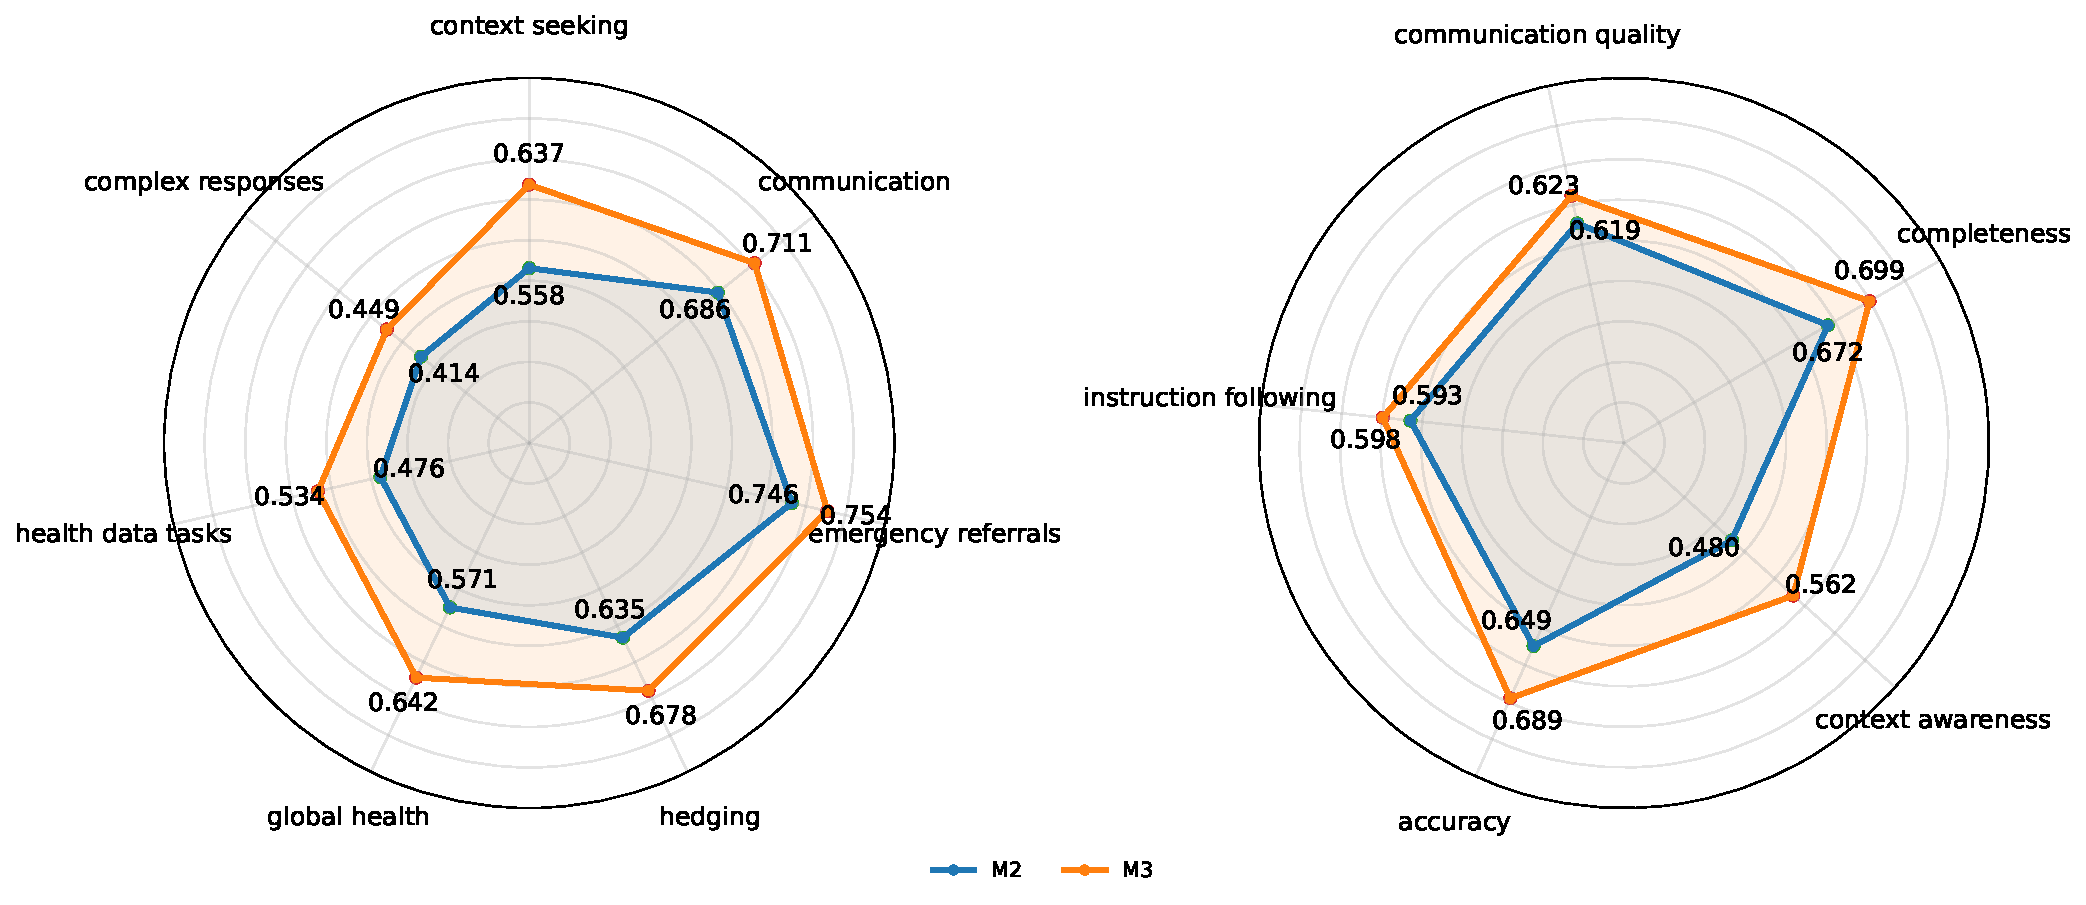
\includegraphics[width=1.0\linewidth]{image/healthbench_radar_m2_vs_m3.pdf}
    \caption{HealthBench fine-grained comparison: M2 vs M3 (themes \& axes).}
    \label{fig:hb_m2_m3}
\end{figure}


% \subsubsection{HB-hard}

\subsubsection{HealthBench-Hallu}

尽管 HealthBench 等基准已为医学 LLM 评估建立了标准，临床安全性仍是医疗 AI 落地的首要考虑。医学幻觉指生成表面合理但事实错误的信息，这一问题已被监管机构与研究社区广泛关注~\cite{ankit2023medhalt, DBLP:journals/corr/abs-2503-05777, DBLP:conf/bionlp/ManesRCBHS24}。该问题在复杂医学推理任务中尤为突出：模型输出通常包含高信息密度的长文本，涵盖精确药物剂量、罕见临床表现等专业知识。长文本生成与语言连贯性相结合，使细粒度事实错误更易逃逸检测，从而带来显著临床风险。因此我们提出 HealthBench-Hallu，一个细粒度评估框架，用于衡量模型在 HealthBench 任务中的事实完整性。该指标通过将输出拆解为原子事实并与外部证据核验，对医学幻觉进行严格量化。


\paragraph{指标设计}

HealthBench-Hallu 关注模型生成内容中的医学事实误解，主要表现为：

\begin{itemize}
    \item \textbf{错误或误用的医学知识：} 叙述错误的临床事实，或将正确知识应用于不恰当语境。
    \item \textbf{伪造或扭曲的医学证据：} 虚构不存在的参考资料、篡改临床数据或捏造因果关系。
\end{itemize}


\paragraph{HealthBench-Hallu 评估}
HealthBench-Hallu 复用事实感知验证流水线（见第~\ref{sec:fact-verifier} 节），但以高精度（而非高吞吐）配置运行：将事实抽取器升级为 GPT-5 以提升细粒度原子事实覆盖，并执行实时多轮检索验证，而非依赖缓存证据。
基于该验证流水线生成的证据标签，我们计算加权幻觉率（$H$）：

\begin{equation}
H = \frac{\sum_{i=1}^{N} w_i}{|\text{Total Claims}|}
\end{equation}

权重 $w_i$ 依据事实风险分层：\textbf{Refuted}（1.0）代表严重事实错误；\textbf{Uncertain}（0.5）代表证据不足或存在歧义风险的陈述；\textbf{Supported}（0.0）代表正确陈述。该指标直接反映模型在复杂医学问题上的可信边界。


\paragraph{实验结果}

表~\ref{tab:hallu_vs_cap} 显示，融合事实感知 RL 使 Baichuan-M3-235B 能够在保留医学推理能力的同时有效抑制幻觉。模型在任务表现上保持竞争力（HealthBench 得分 65.1，与无 RL 变体的 66.2 接近），同时将“被证伪率”和“不确定率”均显著降低约 50\%。这些结果表明，自适应加权策略有效缓解了安全约束与模型效用之间的典型权衡，避免了过度保守方法常见的推理退化。

\begin{table}[htbp]
  \centering
  \caption{Trade-off between hallucination suppression and capability}
    \begin{tabular}{lccc}
    \toprule
    \multicolumn{1}{c}{\textbf{Model}} & \textbf{HealthBench Score} & \textbf{Refuted Rate} & \textbf{Uncertain Rate} \\
    \midrule
    GPT-5.2-High & 63.3  & 2.37\% & 2.78\% \\
    Baichuan-M2-32B & 60.1  & 5.73\% & 5.43\% \\
    M3 - w/o Fact Aware RL & 66.2  & 4.68\% & 3.64\% \\
    \textbf{Baichuan-M3-235B} & \textbf{65.1} & \textbf{2.45\%} & \textbf{2.07\%} \\
    \bottomrule
    \end{tabular}%
  \label{tab:hallu_vs_cap}%
\end{table}%

\paragraph{通过知识探针的幻觉分析}

为阐明事实感知 RL 降低幻觉率的内在机制，我们使用知识探针对模型的\textit{内部认知}（参数化真值）与\textit{外部输出}（生成事实）的一致性进行分析，如图~\ref{fig:Knowledge_Boundary_Alignment} 所示。该分析可通过判断输出是否忠实反映内部参数或因生成不稳定而偏离，从而解耦错误来源。

\begin{figure}[h]
    \centering
    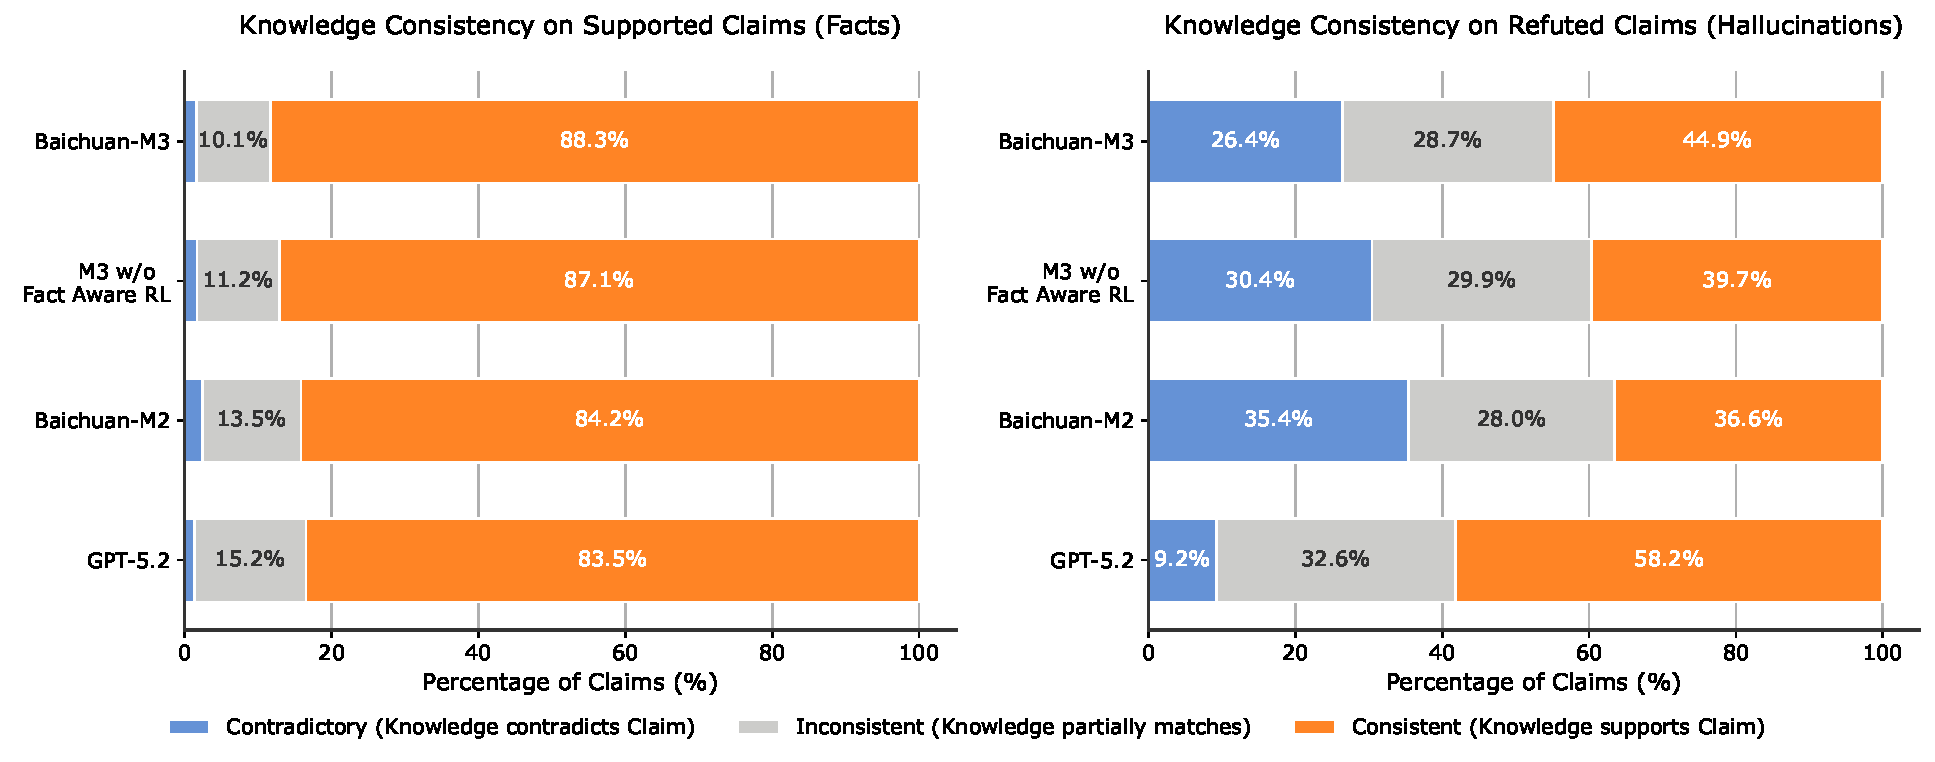
\includegraphics[width=0.98\linewidth]{image/Knowledge_Boundary_Alignment.pdf}
    \caption{\textbf{知识边界一致性分析。} 我们将内部参数与生成事实的一致性划分为三种状态：\textit{一致}（输出与内部认知一致）、\textit{不一致}（部分不匹配）与\textit{矛盾}（输出与内部认知相反）。注意，在幻觉（被证伪事实）情境下，“一致”意味着源于内部知识错误的“诚实错误”。}
    \label{fig:Knowledge_Boundary_Alignment}
\end{figure}

结果显示，事实感知 RL 使模型一致性动态出现明显分化。对于事实正确输出（Supported），内部认知与外部输出的一致性保持在 88.3\%，表明模型的事实真值牢固锚定在内部参数中。更关键的是，对于错误输出（Refuted），一致性显著提升至 44.9\%。这一上升意味着“不忠实幻觉”显著减少——即模型内部认知正确却生成相反错误信息的情形。数据表明剩余幻觉主要是\textit{诚实错误}，即外部输出忠实反映了模型参数中的误解。

最终，这些发现表明事实感知 RL 的主要作用不在于注入新知识，而在于约束模型生成策略，使其严格收敛于自身真实的知识边界内。

